\documentclass[11pt,letterpaper]{article}
\usepackage[T1]{fontenc}
\usepackage{lmodern}
\usepackage{graphicx}
\graphicspath{{./}{../}}
\providecommand{\pandocbounded}[1]{#1}
\usepackage{amsmath,amssymb,mathtools}
\usepackage[margin=1in,top=.85in,bottom=.85in]{geometry}
\usepackage{microtype}
\usepackage{enumitem}
\usepackage{titlesec}
\usepackage{needspace}
\usepackage[hidelinks]{hyperref}
\setlength{\parindent}{0pt}
\setlength{\parskip}{4.5pt plus 1pt minus 1pt}
\setlist{nosep,leftmargin=1.6em,topsep=4pt}
\setlength{\emergencystretch}{1.5em}
\allowdisplaybreaks[1]
\raggedbottom
\widowpenalty=10000
\clubpenalty=10000
\titleformat{\section}{\Large\bfseries}{}{0pt}{}
\titleformat{\subsubsection}{\normalsize\bfseries}{}{0pt}{}
\titleformat{\subsection}{\large\bfseries}{}{0pt}{}
\titlespacing*{\section}{0pt}{14pt}{8pt}
\titlespacing*{\subsubsection}{0pt}{9pt}{4pt}
\titlespacing*{\subsection}{0pt}{12pt}{6pt}
\newcommand{\tightlist}{\setlength{\itemsep}{0pt}\setlength{\parskip}{0pt}}
\hypersetup{pdftitle={Mathematical Analysis - Week
3},pdfsubject={MAT1011 Lecture 8-12 and Tutorial 2}}
\begin{document}
\begin{center}
{\LARGE Mathematical Analysis - Week 3\par}
\vspace{5pt}
{\large Lecture 8-12 and Tutorial 2\par}
\end{center}
\vspace{4pt}
\Needspace{10\baselineskip}
\section{Lecture 8}\label{lecture-8}

\Needspace{8\baselineskip}
\subsection{Derivative at a point}\label{derivative-at-a-point}
\[
\Delta x=h,\quad \Delta y=f(a+h)-f(a),\qquad
\text{secant slope}=\frac{\Delta y}{h}.
\]

\begin{center}
\begin{minipage}{\linewidth}
\centering
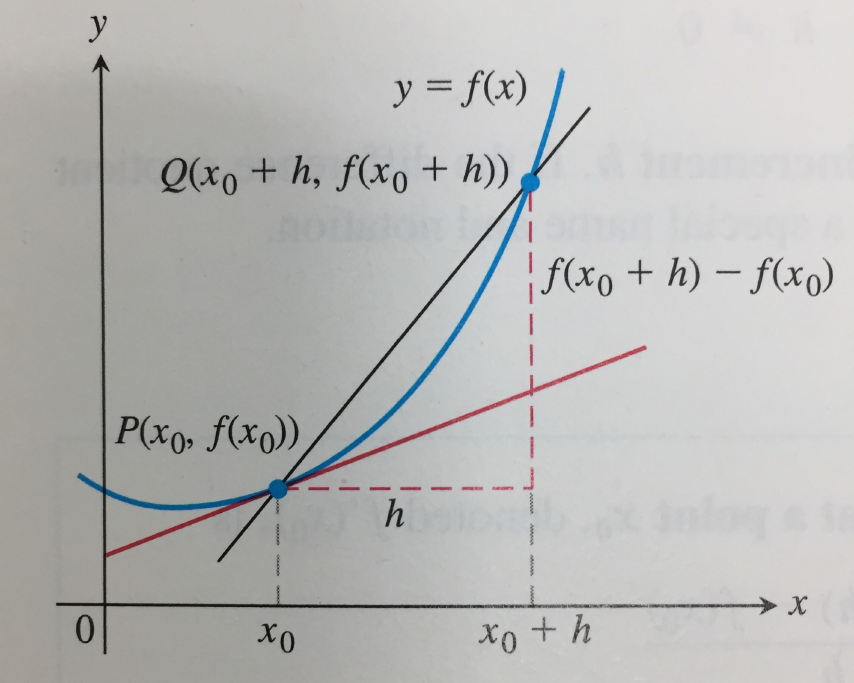
\includegraphics[width=0.36\linewidth,height=\textheight,keepaspectratio]{note-images/w3-secant.png}\par
\vspace{3pt}
{\small \emph{Lecture 8, p.5.}\par}
\end{minipage}
\end{center}

\Needspace{5\baselineskip}
\textbf{Definition 1.2.1.} \(f\) defined on an open interval about
\(a\). If the following limit is finite, \(f\) is differentiable at
\(a\): \[
f'(a)=\lim_{h\to0}\frac{f(a+h)-f(a)}h
=\lim_{x\to a}\frac{f(x)-f(a)}{x-a}.
\] Equivalently, \(\forall\varepsilon>0\ \exists\delta>0\) such that \[
0<|h|<\delta\implies
\left|\frac{f(a+h)-f(a)}h-f'(a)\right|<\varepsilon.
\] Tangent: \(y=f(a)+f'(a)(x-a)\). Other notation: \(y'(a)\),
\(\frac{dy}{dx}(a)\).

\textbf{Ex.1.2.1.} From the definition: \[
\begin{aligned}
\frac{(a+h)^n-a^n}{h}&=na^{n-1}+O(h)\to na^{n-1},\quad n\ge1,\\
\frac{(a+h)^{-2}-a^{-2}}h&=-\frac{2a+h}{a^2(a+h)^2}\to-2a^{-3}\quad(a\ne0),\\
\frac{\sin(a+h)-\sin a}h
&=\sin a\frac{\cos h-1}h+\cos a\frac{\sin h}h\to\cos a.
\end{aligned}
\] Likewise \((\cos x)'=-\sin x\). Radians throughout. Here \(O(h)\)
means a remainder bounded by \(C|h|\) for small \(h\).

\Needspace{8\baselineskip}
\subsection{Oscillation; one-sided
derivatives}\label{oscillation-one-sided-derivatives}

\textbf{Ex.1.2.2.} Extend \(f=x^2\sin(1/x)\) and \(g=x\sin(1/x)\) by
\(f(0)=g(0)=0\).

\begin{center}
\begin{minipage}{\linewidth}
\centering
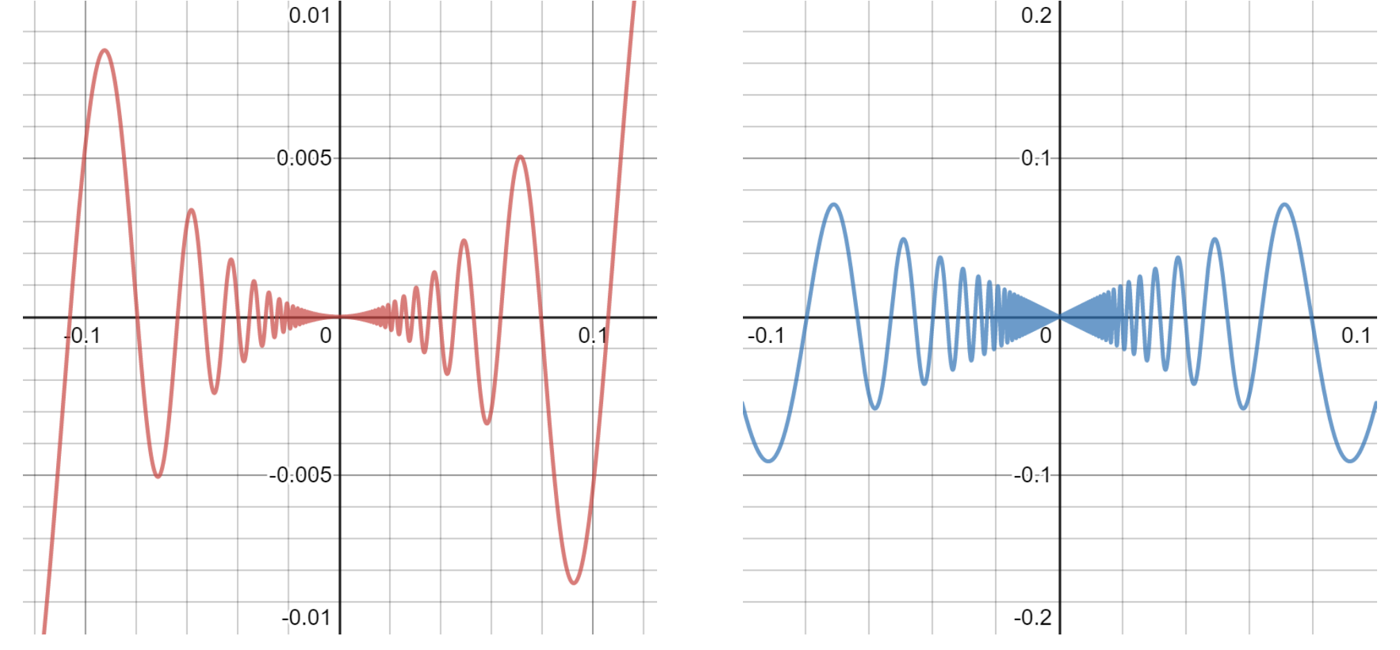
\includegraphics[width=0.78\linewidth,height=\textheight,keepaspectratio]{note-images/w3-oscillation.png}\par
\vspace{3pt}
{\small \emph{Lecture 8, pp.17-18. Left: \(f\); right: \(g\). Different vertical
scales.}\par}
\end{minipage}
\end{center}

Both continuous at \(0\), but \[
\frac{f(h)}h=h\sin(1/h)\to0,\qquad
\frac{g(h)}h=\sin(1/h)\text{ has no limit}.
\] For the second quotient use \(h_n=(\pi/2+2n\pi)^{-1}\) and
\(k_n=(3\pi/2+2n\pi)^{-1}\): values \(1,-1\). Thus \(f'(0)=0\),
\(g'(0)\) undefined. Check the amplitude \textbf{after division by
\(h\)}.

\Needspace{5\baselineskip}
\textbf{Theorem 1.2.2.} Differentiable at \(a\) \(\Rightarrow\)
continuous at \(a\). \[
f(a+h)-f(a)=\frac{f(a+h)-f(a)}h\,h\to f'(a)\cdot0=0.
\] For an explicit estimate: bound the quotient by \(|f'(a)|+1\) for
\(0<|h|<\delta_1\), then take
\(\delta=\min\{\delta_1,\varepsilon/(|f'(a)|+1)\}\).

\Needspace{5\baselineskip}
\textbf{Definition.} \(f'_\pm(a)=\lim_{h\to0^\pm}[f(a+h)-f(a)]/h\). At
an interior point, \(f'(a)\) exists iff both one-sided derivatives are
finite and equal. \[
\begin{array}{c|c|c|c}
f(x)&\text{left quotient limit at }0&\text{right}&\text{shape}\\\hline
|x|&-1&1&\text{corner}\\
\sqrt{|x|}&-\infty&+\infty&\text{cusp}\\
x^{1/3}&+\infty&+\infty&\text{vertical tangent}
\end{array}
\] Infinite limits are not ordinary derivatives. Continuity alone is not
enough.

\Needspace{10\baselineskip}
\section{Tutorial 2}\label{tutorial-2}

\Needspace{8\baselineskip}
\subsection{Algebra and estimates}\label{algebra-and-estimates}

\Needspace{5\baselineskip}
\textbf{Q1.} Cancel/rationalize first: \[
\begin{aligned}
\text{(a)}\quad &\frac{x^3-8}{x^2-4}=\frac{x^2+2x+4}{x+2}\to3\quad(x\to2),\\
\text{(b)}\quad &\frac{\sqrt{1+2x}-\sqrt{1-x}}x
=\frac3{\sqrt{1+2x}+\sqrt{1-x}}\to\frac32\quad(x\to0),\\
\text{(c)}\quad &\frac{x^2\sin(1/x)}{\sqrt{1+x}-1}
=x\sin(1/x)(\sqrt{1+x}+1)\to0,\\
\text{(d)}\quad &\frac{x^n-1}{x^m-1}
=\frac{1+x+\cdots+x^{n-1}}{1+x+\cdots+x^{m-1}}\to\frac nm\quad(x\to1).
\end{aligned}
\] In (c), \(|\text{expression}|\le3|x|\) for \(0<|x|<1/2\).

\Needspace{5\baselineskip}
\textbf{Q4(a).} For \(x_0\ne0\), first impose \(|x-x_0|<|x_0|/2\), so
\(|x|>|x_0|/2\). \[
\left|\frac1x-\frac1{x_0}\right|\le\frac{2|x-x_0|}{|x_0|^2};\qquad
\delta=\min\left\{\frac{|x_0|}2,\frac{\varepsilon|x_0|^2}2\right\}.
\]

\Needspace{5\baselineskip}
\textbf{Q4(b).} Write \(1/x=\lfloor1/x\rfloor+r\), \(0\le r<1\). Then \[
\left|x\lfloor1/x\rfloor-1\right|=|xr|\le|x|\to0.
\] Limit \(1\); \(\delta=\varepsilon\). Works for negative \(x\) too.

\Needspace{5\baselineskip}
\textbf{Q2.} Let \(H=f/x^2\to1\) as \(x\to0\). Eventually \(|H|<2\),
hence \[
|f/x|<2|x|\to0,\qquad |f|<2x^2\to0.
\] If \(|H-1|<1\) for \(0<|x|<\delta_1\), use respectively
\(\min\{\delta_1,\varepsilon/2\}\) and
\(\min\{\delta_1,\sqrt{\varepsilon/2}\}\).

Also \(H>1/2\) near \(0\), so \(f>0\) there and \[
\frac{\sqrt f}{|x|}=\sqrt H,\qquad
|\sqrt H-1|=\frac{|H-1|}{\sqrt H+1}\le|H-1|\to0.
\] Limit \(1\). Use a common radius for \(H>1/2\) and
\(|H-1|<\varepsilon\). Remember \(\sqrt{x^2}=|x|\).

\Needspace{8\baselineskip}
\subsection{Quantifiers}\label{quantifiers}

\Needspace{5\baselineskip}
\textbf{Q3(a).} Wrong: \(\forall\varepsilon\ \forall\delta\ \exists x\)
with both inequalities true. Only asks for one good point. Correct: \[
\forall\varepsilon>0\ \exists\delta>0\ \forall x\in\operatorname{dom}f:
\quad 0<|x-c|<\delta\implies |f(x)-L|<\varepsilon.
\] Counterexample to the wrong definition: \(f(x)=\sin(1/x)\),
\(c=L=0\). Every neighborhood contains \(x=1/(n\pi)\) with \(f(x)=0\).

\Needspace{5\baselineskip}
\textbf{Q3(b).} Negation for a fixed candidate \(L\): \[
\exists\varepsilon_0>0\ \forall\delta>0\ \exists x\in\operatorname{dom}f:
\quad 0<|x-c|<\delta,\quad |f(x)-L|\ge\varepsilon_0.
\] To show no finite limit, do this for \textbf{every}
\(L\in\mathbb R\). For \(\sin(1/x)\) choose \(\varepsilon_0=1\): if
\(L\le0\), use points with sine \(1\); if \(L>0\), use sine \(-1\). Such
points occur arbitrarily close to \(0\).

\Needspace{5\baselineskip}
\textbf{Q5(a): uniqueness.} If \(f\to A,B\) and \(A\ne B\), choose
\(\varepsilon=|A-B|/3\) and a common radius. Then \[
|A-B|\le|A-f(x)|+|f(x)-B|<2|A-B|/3,
\] contradiction.

\Needspace{5\baselineskip}
\textbf{Q5(b).} \(f=g\) for \(0<|x-c|<r\) \(\Rightarrow\) same limit at
\(c\). Use \(\delta=\min\{r,\delta_f\}\). The value at \(c\) is
irrelevant.

\Needspace{5\baselineskip}
\textbf{Q5(c).} \(f\to A\Rightarrow|f|\to|A|\), since \[
\bigl||f|-|A|\bigr|\le|f-A|.
\] Converse holds for all \(f\) when \(A=0\). For \(A\ne0\), take
\(f=|A|\) to the right of \(c\), \(f=-|A|\) to the left.

\Needspace{8\baselineskip}
\subsection{Density and coupled
limits}\label{density-and-coupled-limits}

\Needspace{5\baselineskip}
\textbf{Q6.} \(D=1\) on \(\mathbb Q\), \(0\) otherwise; \(F(x)=xD(x)\).

At \(0\): \(|F(x)|\le|x|\to0\). At \(x_0\ne0\), suppose \(F\to L\). Take
\(\varepsilon=|x_0|/4\) and \(\delta\le|x_0|/4\) within the limit
radius. Density gives rational \(q\) and irrational \(t\) in that
punctured neighborhood. Then \[
\frac34|x_0|<|q|=|F(q)-F(t)|<2\varepsilon=\frac12|x_0|,
\] contradiction. Limit exists only at \(0\).

\Needspace{5\baselineskip}
\textbf{Q7.} \(f<g\), \(f\to A\), \(g\to B\) \(\Rightarrow A\le B\).

If \(A>B\), use \(\varepsilon=(A-B)/3\): near \(c\),
\(f>A-\varepsilon>B+\varepsilon>g\), impossible. Strictness may
disappear: \(0<x^2\) for \(x\ne0\), both limits \(0\).

\Needspace{5\baselineskip}
\textbf{Q8.} Assume \(S=f+g\to0\), \(P=fg\to0\). Key identity: \[
0\le f^2+g^2=S^2-2P\le|S|^2+2|P|.
\] Given \(\varepsilon>0\), choose a common radius with
\(|S|<\varepsilon/\sqrt2\), \(|P|<\varepsilon^2/4\). Then
\(f^2+g^2<\varepsilon^2\), so \(|f|,|g|<\varepsilon\). Both tend to
\(0\).

Do not assume the individual limits exist first. Need both hypotheses:
\((f,g)=(1,-1)\) or \((0,1)\) shows what happens if one is dropped.

\Needspace{8\baselineskip}
\subsection{Substitutions; derivatives at
zero}\label{substitutions-derivatives-at-zero}

\Needspace{5\baselineskip}
\textbf{Q9(a).} \(h=x-x_0\): same radius in \[
\lim_{x\to x_0}f(x)=A\iff\lim_{h\to0}f(x_0+h)=A.
\] \textbf{Q9(b).} If \(f(x)\to A\) at \(0\), then \(f(t^2)\to A\): use
\(|t|<\sqrt\delta\). Converse fails: \(f=1\) for \(x>0\), \(0\) for
\(x<0\). Squaring only sees the right side.

\Needspace{5\baselineskip}
\textbf{Q10.} \(F=x\sin x\cos(1/x)\) off \(0\), \(F(0)=0\): \[
|F(h)/h|=|\sin h\cos(1/h)|\le|h|\to0;\quad F'(0)=0.
\] \textbf{Q11.} \(G=(\sqrt{1+x^2}-1)/x\) off \(0\), \(G(0)=0\): \[
\frac{G(h)}h=\frac1{\sqrt{1+h^2}+1}\to\frac12;\quad G'(0)=\frac12.
\]

\Needspace{5\baselineskip}
\textbf{Q12: fixed point.} Continuous \(f:[0,1]\to[0,1]\). Set
\(H=f-x\): \[
H(0)\ge0,\quad H(1)\le0\quad\xRightarrow{\mathrm{IVT}}\quad
H(c)=0\text{ for some }c\in[0,1].
\] If \(f\) is strictly decreasing, two fixed points \(c_1<c_2\) would
give \(c_1=f(c_1)>f(c_2)=c_2\). Unique. Without this, \(f(x)=x\) fixes
everything.

\Needspace{5\baselineskip}
\textbf{Q13.} For \(f>0\) on a punctured neighborhood, \[
f\to+\infty\iff1/f\to0.
\] Forward: use threshold \(M=1/\varepsilon\). Reverse: use error
\(\varepsilon=1/M\), giving \(0<1/f<1/M\Rightarrow f>M\). Positivity
matters: \(f=-(x-c)^{-2}\) has \(1/f\to0\) but \(f\to-\infty\).

\Needspace{10\baselineskip}
\section{Lecture 9}\label{lecture-9}

\Needspace{8\baselineskip}
\subsection{Rules and compositions}\label{rules-and-compositions}

For differentiable \(u,v\): \[
\begin{aligned}
(cu)'&=cu',&(u+v)'&=u'+v',\\
(uv)'&=u'v+uv',&(u/v)'&=(u'v-uv')/v^2\quad(v\ne0).
\end{aligned}
\] Product rule: insert \(u(x+h)v(x)\) in the numerator: \[
\frac{\Delta(uv)}h
=u(x+h)\frac{\Delta v}h+v(x)\frac{\Delta u}h\to uv'+vu'.
\] Reciprocal: \(\Delta(1/v)/h=-[v(x+h)v(x)]^{-1}\Delta v/h\).

\textbf{Ex.1.2.4.} \((\tan x)'=\sec^2x\), \((\cot x)'=-\csc^2x\) on
their domains; \((x^2\sin x)'=2x\sin x+x^2\cos x\).

\Needspace{5\baselineskip}
\textbf{Theorem 1.2.3 (Chain rule).} \(g\) differentiable at \(a\),
\(f\) at \(g(a)\): \[
(f\circ g)'(a)=f'(g(a))g'(a).
\] The cancellation
\(\Delta y/\Delta x=(\Delta y/\Delta u)(\Delta u/\Delta x)\) misses
\(\Delta u=0\). Proof repaired in Lecture 10.

\textbf{Ex.1.2.5.} \[
\begin{aligned}
(\sin(1/x))'&=-\cos(1/x)/x^2\quad(x\ne0),\\
[\sin(\sin(\sin x))]'&=\cos(\sin(\sin x))\cos(\sin x)\cos x.
\end{aligned}
\] For \(y=\sqrt{x+\sqrt{x+\sqrt x}}\), name the layers (\(x>0\)): \[
r=\sqrt x,\ s=\sqrt{x+r},\ y=\sqrt{x+s};\qquad
r'=\frac1{2r},\ s'=\frac{1+r'}{2s},\ y'=\frac{1+s'}{2y}.
\] At a join, use the definition: \(q=x^{3/2}\) for \(x\ge0\), \(q=x^2\)
for \(x<0\). Quotients at \(0\): \(\sqrt h\) on the right, \(h\) on the
left, hence \(q'(0)=0\).

\textbf{Ex.1.2.6.} For the earlier \(f=x^2\sin(1/x)\), extended by
\(0\), \[
f'(x)=\begin{cases}2x\sin(1/x)-\cos(1/x),&x\ne0,\\0,&x=0.\end{cases}
\] \(f'\) is discontinuous at \(0\): values \(-1,1\) at
\(1/(2n\pi),1/((2n+1)\pi)\). Differentiable does not mean continuously
differentiable.

\Needspace{8\baselineskip}
\subsection{Higher derivatives}\label{higher-derivatives}

\(f^{(0)}=f\), \(f^{(n)}=(f^{(n-1)})'\); \(d^2y/dx^2\ne(dy/dx)^2\). For
integers \(m\ge1\), \(n\ge0\): \[
\begin{aligned}
D^n x^m&=\begin{cases}\dfrac{m!}{(m-n)!}x^{m-n},&0\le n\le m,\\0,&n>m,\end{cases}\\
D^n\sin x&=\sin(x+n\pi/2),\qquad D^n\cos x=\cos(x+n\pi/2).
\end{aligned}
\] \textbf{Leibniz (Ex.1.2.8).} For \(n\)-times differentiable \(f,g\),
\[
(fg)^{(n)}=\sum_{k=0}^n\binom nk f^{(n-k)}g^{(k)}.
\] Induction: differentiate, shift the second sum, combine using
\(\binom nk+\binom n{k-1}=\binom{n+1}k\).

For \(n\ge2\), only three terms survive in \(D^n(x^2\sin x)\): \[
x^2\sin(x+n\pi/2)+2nx\sin(x+(n-1)\pi/2)
+n(n-1)\sin(x+(n-2)\pi/2).
\] \textbf{Ex.1.2.9.} Writing \(f'(g)=f'(g(x))\), \[
\begin{aligned}
y''&=f''(g)(g')^2+f'(g)g'',\\
y'''&=f'''(g)(g')^3+3f''(g)g'g''+f'(g)g'''.
\end{aligned}
\]

\Needspace{8\baselineskip}
\subsection{Implicit differentiation}\label{implicit-differentiation}

Assume \(y=y(x)\) differentiable on the branch being used. Remember the
\(y'\) factors.

\textbf{Ex.1.2.10.} \[
\begin{aligned}
x^2+y^2=1&\implies2x+2yy'=0\implies y'=-x/y\quad(y\ne0),\\
y^2=x^2+\sin(xy)&\implies(2y-x\cos(xy))y'=2x+y\cos(xy).
\end{aligned}
\] Solve the second equation only when the coefficient of \(y'\) is
nonzero.

Inverse functions, assuming both differentiable: \(g(f(x))=x\) gives
\(f'=1/(g'\circ f)\). In particular \((\arcsin x)'=1/\sqrt{1-x^2}\) for
\(|x|<1\).

\textbf{Ex.1.2.11.} \(x^3+y^3=9xy\) at \((2,4)\): \[
y'=\frac{3y-x^2}{y^2-3x}=\frac45;\quad
\text{tangent }y-4=\tfrac45(x-2),\quad
\text{normal }y-4=-\tfrac54(x-2).
\] \textbf{Ex.1.2.12.} \(F(x)+G(xy)+H(y^2)=0\): \[
F'(x)+G'(xy)(y+xy')+2yH'(y^2)y'=0,
\] so \(y'=-[F'(x)+yG'(xy)]/[xG'(xy)+2yH'(y^2)]\) if the denominator is
nonzero.

\textbf{Ex.1.2.13.} \(2x^3-3y^2=8\): \(y'=x^2/y\), \(y''=2x/y-x^4/y^3\)
(\(y\ne0\)).

For \(y^4-2y^2=x^4-3x^2\), set \(A=4y^3-4y\), \(B=4x^3-6x\): \[
Ay'=B\implies(12y^2-4)(y')^2+Ay''=12x^2-6.
\] Less work than differentiating the quotient. Divide by \(A\) only if
\(A\ne0\).

\Needspace{8\baselineskip}
\subsection{A few exercises}\label{a-few-exercises}

\(a\) fixed: \([g(x+g(a))]'=g'(x+g(a))\), but
\([g(x+g(x))]'=g'(x+g(x))(1+g'(x))\). For \(g\circ g\circ g\), multiply
the three derivative factors.

\(p=x(x-1)\cdots(x-1000)=xq\): \(p'(0)=q(0)=1000!\). Do not expand.

If \(\varphi\) is continuous at \(a\): \[
[(x-a)\varphi(x)]'_{x=a}=\lim_{h\to0}\varphi(a+h)=\varphi(a).
\] For \(|x-a|\varphi(x)\), right/left derivatives are
\(\varphi(a),-\varphi(a)\); differentiable iff \(\varphi(a)=0\).

If \(g(0)=g'(0)=0\) and \(f(x)=g(x)\sin(1/x^2)\) off \(0\), \(f(0)=0\):
\[
|f(h)/h|\le|g(h)/h|\to0\implies f'(0)=0.
\] Even continuous \(g'\) does not force continuous \(f'\): for
\(g=x^2\), \[
f'(x)=2x\sin(1/x^2)-2\cos(1/x^2)/x
\] is unbounded near \(0\).

\Needspace{10\baselineskip}
\section{Lecture 10}\label{lecture-10}

\Needspace{8\baselineskip}
\subsection{Linearization and
differentials}\label{linearization-and-differentials}

For differentiable \(f\) at \(a\), set
\(\eta(h)=[f(a+h)-f(a)]/h-f'(a)\to0\). Then \[
f(a+h)=f(a)+f'(a)h+\eta(h)h.
\] \textbf{Definition.} \(L(x)=f(a)+f'(a)(x-a)\) is the linearization.
Error \(o(|h|)\) means \[
\frac{|f(a+h)-L(a+h)|}{|h|}\to0.
\] Exact equality with the remainder; approximation only after dropping
it.

\textbf{Ex.1.2.14: best line.} \(P=(a,f(a))\), \(Q=(a+h,f(a+h))\). For
the line \(L_m\) through \(P\) with slope \(m\), \[
\frac{\operatorname{dist}(Q,L_m)}{\operatorname{dist}(Q,P)}
=\frac{|[f(a+h)-f(a)]/h-m|}
{\sqrt{1+m^2}\sqrt{1+([f(a+h)-f(a)]/h)^2}}
\to\frac{|f'(a)-m|}{\sqrt{1+m^2}\sqrt{1+f'(a)^2}}.
\] Zero iff \(m=f'(a)\). For the vertical line the limit is
\(1/\sqrt{1+f'(a)^2}>0\). Hence only the tangent has relative distance
tending to zero.

\Needspace{5\baselineskip}
\textbf{Definition (Differential).} \(dx\) independent; \(dy=f'(a)dx\).
With \(dx=h\), \[
\Delta y=f(a+h)-f(a),\qquad \Delta y=dy+o(|h|).
\]

\begin{center}
\begin{minipage}{\linewidth}
\centering
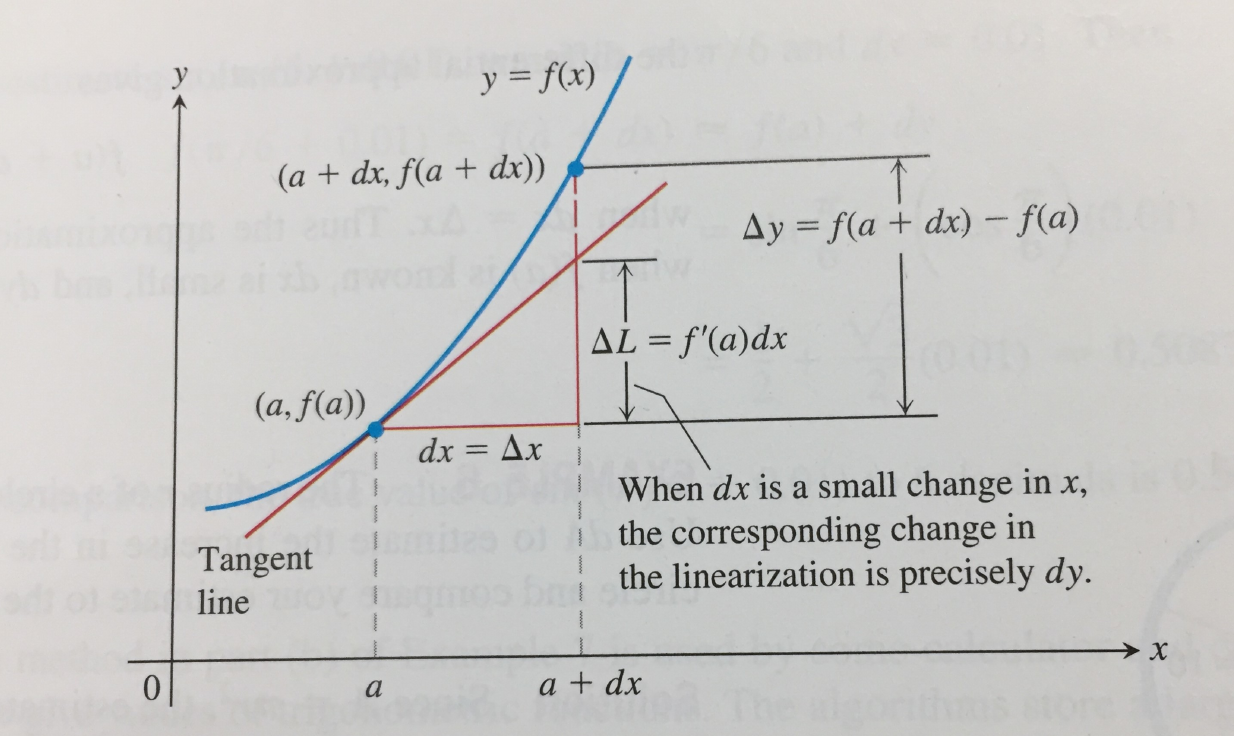
\includegraphics[width=0.5\linewidth,height=\textheight,keepaspectratio]{note-images/w3-differential.png}\par
\vspace{3pt}
{\small \emph{Lecture 10, p.27. Curve change \(\Delta y\); tangent change
\(dy=\Delta L\).}\par}
\end{minipage}
\end{center}

\textbf{Ex.1.2.17.} \(f=\sqrt{1+x}\) at \(0\): \(dy=dx/2\) and \[
\Delta y-dy=\sqrt{1+h}-1-h/2
=-\frac{h^2}{2(\sqrt{1+h}+1)^2},\qquad
|\Delta y-dy|\le h^2/4\quad(|h|<1/2).
\] Thus \(\sqrt{1.02}\approx1.01\), error \(\le10^{-4}\); overestimate.

\textbf{Ex.1.2.18.} At \(0\):

\begin{itemize}
\tightlist
\item
  \(x^2\sin(1/x)\), extended by \(0\): derivative \(0\), differential
  \(0\).
\item
  \(x^2D(x)\): quotient \(hD(h)\to0\), differential \(0\); discontinuous
  at every nonzero point.
\item
  \(u=x\) on rationals, \(\sin x\) otherwise: quotient \(1\) or
  \(\sin h/h\to1\), so \(du=dx\).
\end{itemize}

\Needspace{8\baselineskip}
\subsection{Increment form; chain rule
proof}\label{increment-form-chain-rule-proof}

\textbf{Ex.1.2.19-20.} In one variable, \[
f\text{ differentiable at }a
\iff f(a+h)-f(a)=Ah+\eta(h)h,\quad\eta(h)\to0.
\] Forward: define \(\eta\) as above, \(A=f'(a)\). Reverse: divide by
\(h\); quotient \(\to A\), so \(f'(a)=A\).

For the chain rule, \(u_0=g(a)\), \(k=\Delta u\): \[
\begin{aligned}
\Delta u&=(g'(a)+\beta(h))h,\quad\beta(h)\to0,\\
f(u_0+k)-f(u_0)&=(f'(u_0)+\alpha(k))k,\quad\alpha(k)\to0.
\end{aligned}
\] Set \(\alpha(0)=0\). Since \(\Delta u\to0\), \[
\frac{f(g(a+h))-f(g(a))}{h}
=(f'(u_0)+\alpha(\Delta u))(g'(a)+\beta(h))\to f'(u_0)g'(a).
\] No division by \(\Delta u\); the missing case is included.

\textbf{\(C^1\) reminder.} \(f''\) exists \(\Rightarrow f\in C^1\)
(\(f'\) continuous) \(\Rightarrow f\) differentiable \(\Rightarrow f\)
continuous, on an open interval. Converses fail at \(0\), respectively:
\(x|x|\), \(x^2\sin(1/x)\) extended by \(0\), \(|x|\).

\newpage

\Needspace{10\baselineskip}
\section{Lecture 11}\label{lecture-11}

\Needspace{8\baselineskip}
\subsection{Extreme values}\label{extreme-values}

\Needspace{5\baselineskip}
\textbf{Definition.} Absolute maximum at \(c\in D\): \(f(x)\le f(c)\)
for all \(x\in D\). Minimum: reverse inequality. Supremum need not be
attained.

\textbf{Ex.1.2.22.}

\begin{itemize}
\tightlist
\item
  \(x\) on \((0,1)\): neither extremum. \(\arctan x\) on \(\mathbb R\):
  neither; bounds \(\pm\pi/2\) not attained.
\item
  \(f=|x|\) for \(0<|x|<1\), \(f(0)=f(\pm1)=1/2\): on \([-1,1]\), inf
  \(0\), sup \(1\), neither attained.
\item
  \(u(p/q)=1/q\), reduced, \(q>0\): max \(1\), no minimum. Giving
  irrationals value \(1\) on \([0,1]\) still gives max \(1\), no
  minimum.
\end{itemize}

\Needspace{5\baselineskip}
\textbf{Theorem 1.2.4 (EVT).} Continuous on \([a,b]\) \(\Rightarrow\)
attains both absolute extrema. Need continuity + closed + bounded.

\emph{Proof sketch.} Unbounded \(f\) would give \(|f(x_n)|>n\). A
subsequence \(x_{n_j}\to c\in[a,b]\) contradicts continuity. Thus
\(M=\sup f\) is finite. Choose \[
M-1/n<f(x_n)\le M.
\] Take a convergent subsequence again: \(f(c)=M\). Apply to \(-f\) for
the minimum. Uses the bounded-sequence subsequence theorem.

\Needspace{5\baselineskip}
\textbf{Definition.} Local maximum at \(c\in D\): for some \(\delta>0\),
\[
f(x)\le f(c)\quad(x\in D\cap(c-\delta,c+\delta)).
\] Strict: \(<\) for \(x\ne c\). Endpoints count relative to \(D\).

\begin{center}
\begin{minipage}{\linewidth}
\centering
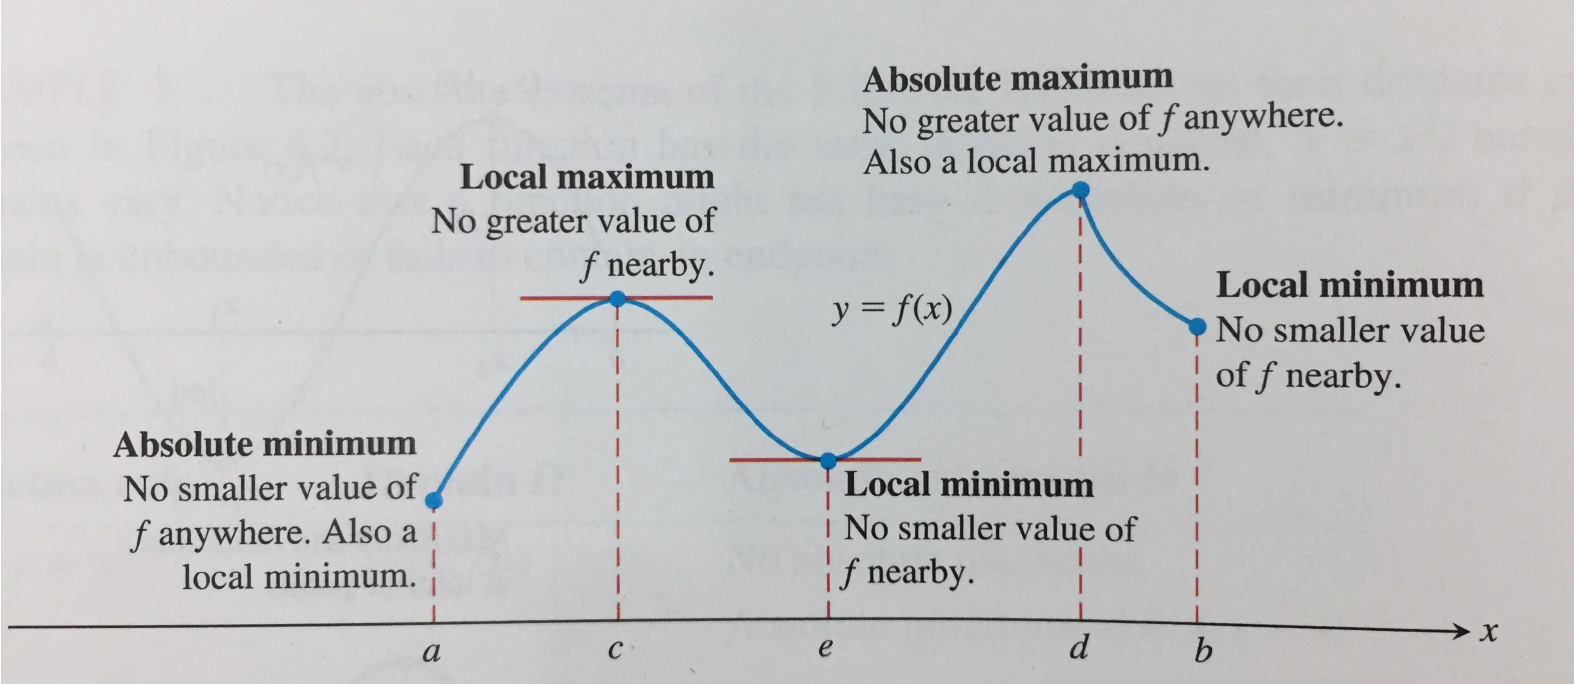
\includegraphics[width=0.65\linewidth,height=\textheight,keepaspectratio]{note-images/w4-local-global.png}\par
\vspace{3pt}
{\small \emph{Lecture 11, p.17.}\par}
\end{minipage}
\end{center}

\Needspace{5\baselineskip}
\textbf{Theorem 1.2.5 (Fermat).} Interior local extremum +
differentiable \(\Rightarrow f'(c)=0\).

At a local maximum, \[
h>0:\ \frac{f(c+h)-f(c)}h\le0,\qquad
h<0:\ \frac{f(c+h)-f(c)}h\ge0.
\] Same limit \(\Rightarrow f'(c)=0\). Minimum: apply to \(-f\).

\textbf{Critical point:} interior point with \(f'=0\) or \(f'\)
undefined. Only a candidate: \(x^3\) at \(0\) has no extremum; \(|x|\)
has a minimum but no derivative. Endpoints checked separately (\(x\) on
\([0,1]\)).

\Needspace{8\baselineskip}
\subsection{Refraction}\label{refraction}

\textbf{Ex.1.2.27.} \(A=(0,a)\), \(B=(d,-b)\), crossing point
\(P=(x,0)\); \(a,b,d,c_1,c_2>0\).

\begin{center}
\begin{minipage}{\linewidth}
\centering
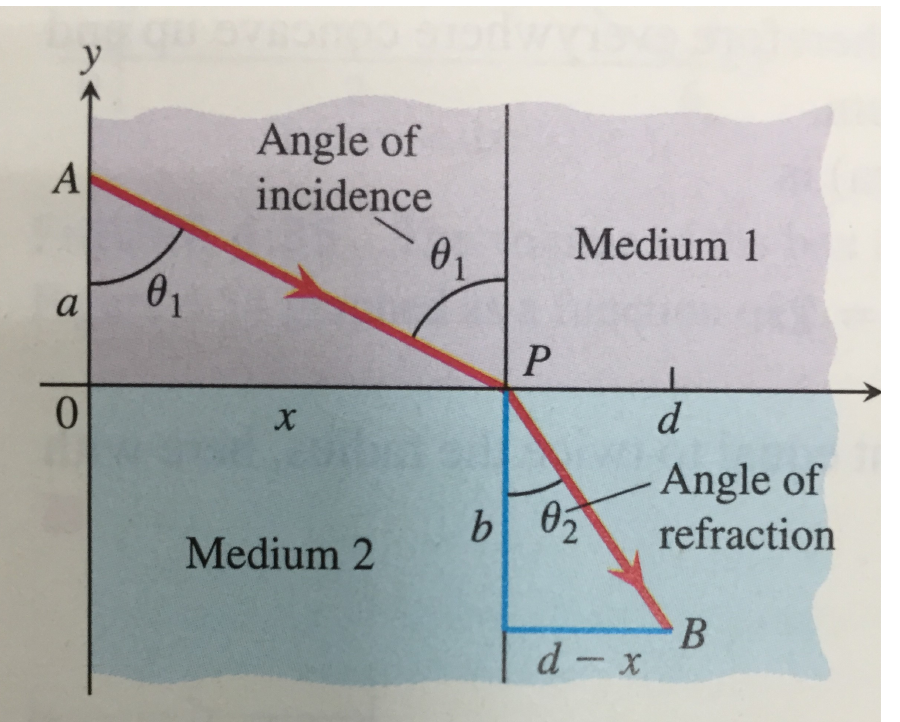
\includegraphics[width=0.36\linewidth,height=\textheight,keepaspectratio]{note-images/w4-refraction.png}\par
\vspace{3pt}
{\small \emph{Lecture 11, p.37. Angles from the normal.}\par}
\end{minipage}
\end{center}

Minimize time, not length: \[
T(x)=\frac{\sqrt{a^2+x^2}}{c_1}+\frac{\sqrt{b^2+(d-x)^2}}{c_2},\quad0\le x\le d.
\] \(T'(0)<0<T'(d)\), so the EVT minimum is interior. Fermat gives \[
T'(x)=\frac{x}{c_1\sqrt{a^2+x^2}}-\frac{d-x}{c_2\sqrt{b^2+(d-x)^2}}=0
\implies\frac{\sin\theta_1}{c_1}=\frac{\sin\theta_2}{c_2}.
\] Unique:
\(T''=a^2/[c_1(a^2+x^2)^{3/2}]+b^2/[c_2(b^2+(d-x)^2)^{3/2}]>0\).

\Needspace{8\baselineskip}
\subsection{Rolle and MVT}\label{rolle-and-mvt}

\Needspace{5\baselineskip}
\textbf{Theorem 1.2.6 (Rolle).} \(f\in C[a,b]\), differentiable on
\((a,b)\), \(f(a)=f(b)\) \(\Rightarrow\exists c\in(a,b)\) with
\(f'(c)=0\).

Proof: constant case immediate. Otherwise an absolute max or min differs
from the endpoint value, hence lies inside. EVT + Fermat.

\begin{center}
\begin{minipage}{\linewidth}
\centering
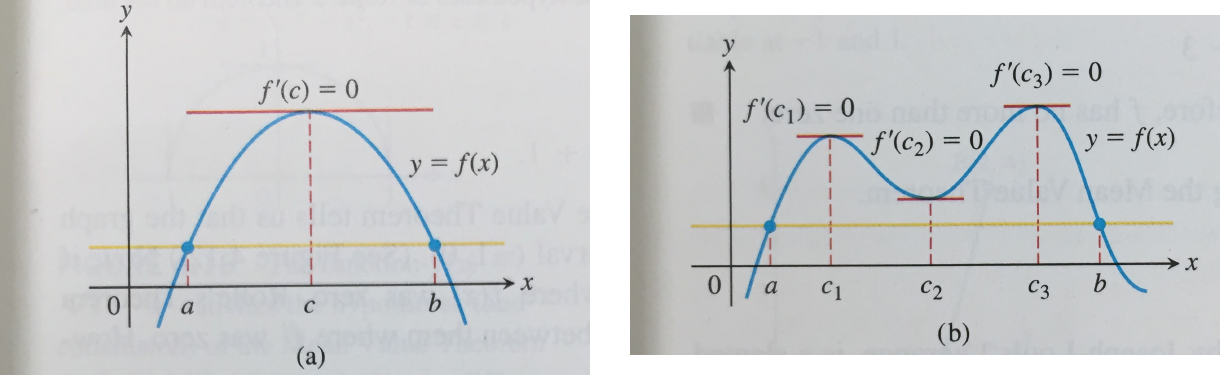
\includegraphics[width=0.65\linewidth,height=\textheight,keepaspectratio]{note-images/w4-rolle.png}\par
\vspace{3pt}
{\small \emph{Lecture 11, p.43. At least one, not necessarily one.}\par}
\end{minipage}
\end{center}

No endpoint derivatives required. Interior differentiability matters:
\(|x|\) on \([-1,1]\) is a counterexample without it.

\Needspace{5\baselineskip}
\textbf{Theorem 1.2.7 (MVT).} \(f\in C[a,b]\), differentiable on
\((a,b)\): \[
\exists c\in(a,b):\qquad f(b)-f(a)=f'(c)(b-a).
\] Subtract the secant: \(h(x)=f(x)-f(a)-\frac{f(b)-f(a)}{b-a}(x-a)\).
Then \(h(a)=h(b)=0\); Rolle gives the result.

\Needspace{5\baselineskip}
\textbf{Corollary 1.2.8.} \(f'=0\) on an interval \(\Rightarrow f\)
constant. Apply MVT between any two points. Disconnected domains may
have different constants on different pieces.

\textbf{Ex.1.2.29.} \(F=x^{100}-x-1\): \(F(1)=-1\) and \[
F(1+t)>99t-1\ (t>0)\implies F(100/99)>0.
\] IVT gives a root in \((1,100/99)\); \(F'=100x^{99}-1>0\) there gives
uniqueness by Rolle.

\textbf{Ex.1.2.31.} \(F=x^2-\sin x\): root \(0\), and another in
\((\pi/6,1)\) since \(F(\pi/6)<0<F(1)\). Three roots would give two
zeros of \(F'\) and one of \(F''\), but \(F''=2+\sin x\ge1\). Exactly
two roots.

\textbf{Ex.1.2.32.} If \(f''\) is continuous on \([a-\delta,a+\delta]\),
set \(M=\max|f''|\). MVT twice, for \(0<|h|<\delta\): \[
\Delta y-dy=[f'(\xi)-f'(a)]h=f''(\eta)(\xi-a)h
\implies |\Delta y-dy|\le M|h|^2.
\] \(\xi,\eta\) lie between \(a\) and \(a+h\).

\textbf{Ex.1.2.33.} \(f\in C[a,b]\), differentiable inside;
\(f'(x)\to L\in\mathbb R\) as \(x\to a^+\). Then \[
\frac{f(x)-f(a)}{x-a}=f'(c_x),\quad a<c_x<x;\qquad c_x\to a^+\implies f'_+(a)=L.
\]

\Needspace{10\baselineskip}
\section{Lecture 12}\label{lecture-12}

\Needspace{8\baselineskip}
\subsection{Monotonicity and extrema
tests}\label{monotonicity-and-extrema-tests}

Strict increase: \(u<v\Rightarrow f(u)<f(v)\); nondecrease: \(\le\)
instead.

\textbf{Ex.1.2.34.} For \(f\in C[a,b]\), differentiable inside, \[
f(v)-f(u)=f'(c)(v-u).
\] Thus \(f'>0\) gives strict increase; \(f'\ge0\) gives nondecrease.
Reverse signs for decrease. Strict increase need not mean \(f'>0\)
everywhere: \(x^3\).

\Needspace{5\baselineskip}
\textbf{Proposition 1.2.9 (First derivative test).} \(f\) continuous
near \(c\), differentiable on either side: \[
\begin{array}{c|c|c}
f'\text{ on left}&f'\text{ on right}&c\\\hline
-&+&\text{strict minimum}\\
+&-&\text{strict maximum}\\
+&+&\text{neither}\\
-&-&\text{neither}
\end{array}
\] Proof: MVT on \([x,c]\) or \([c,x]\) compares \(f(x)\) with \(f(c)\).
No derivative at \(c\) needed.

\Needspace{5\baselineskip}
\textbf{Theorem 1.2.10 (Second derivative test).} \(f''\) continuous
near \(c\), \(f'(c)=0\): \[
f''(c)>0\Rightarrow\text{strict min},\qquad f''(c)<0\Rightarrow\text{strict max}.
\] E.g. \(f''>0\) nearby makes \(f'\) strictly increasing through \(0\);
use the first test. If \(f''(c)=0\): inconclusive (\(x^4,-x^4,x^3\)).

\textbf{Ex.1.2.36.} \(f=x^2(2+\sin(1/x))\), extended by \(f(0)=0\): \[
f(x)\ge x^2>0\ (x\ne0),\quad f'(0)=0,\quad
f'(x)=2x(2+\sin(1/x))-\cos(1/x)\ (x\ne0).
\]

\begin{center}
\begin{minipage}{\linewidth}
\centering
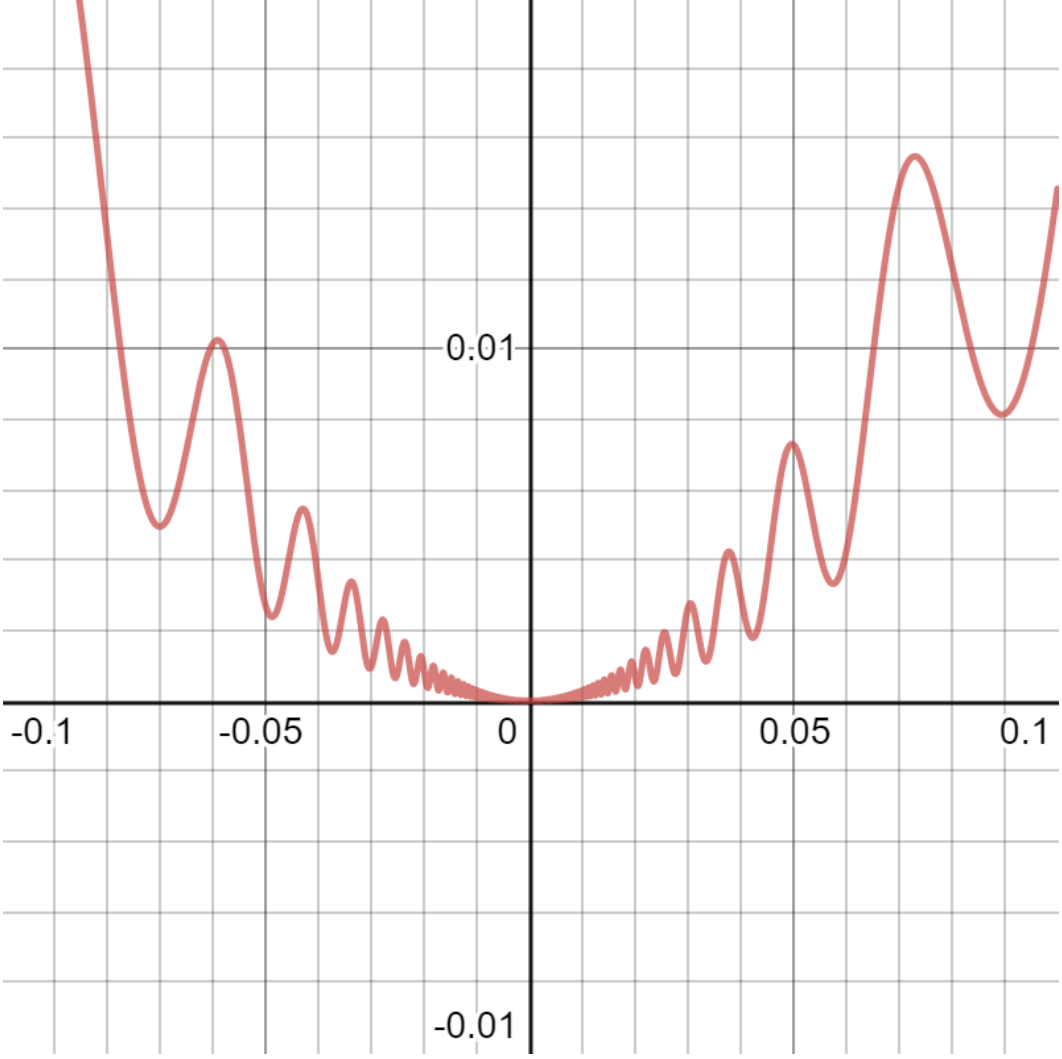
\includegraphics[width=0.4\linewidth,height=\textheight,keepaspectratio]{note-images/w4-oscillation.png}\par
\vspace{3pt}
{\small \emph{Lecture 12, p.13.}\par}
\end{minipage}
\end{center}

Strict minimum at \(0\), but no monotone neighborhood on either side. At
\(1/(2n\pi)\), \(f'<0\) eventually; at \(1/((2n+1)\pi)\), \(f'>0\).
Negative sequences give both signs too. The first-test sign pattern is
sufficient, not necessary.

\textbf{Ex.1.2.24 revisited.} \(f=(x-1)x^{2/3}\): \[
f'=\frac{5x-2}{3x^{1/3}},\quad
\begin{array}{c|ccc}
x&(-\infty,0)&(0,2/5)&(2/5,\infty)\\\hline
f'&+&-&+
\end{array}
\] Local max at \(0\); local min at \(2/5\), value
\(-\frac35(2/5)^{2/3}\) (correcting the slide typo).

\textbf{Ex.1.2.37.} \(f=|2x^3-9x^2+12x|\) on \([-1/4,5/2]\). Since
\(2x^2-9x+12>0\), split at \(0\): \[
f'=\begin{cases}-6(x-1)(x-2),&x<0,\\6(x-1)(x-2),&x>0.\end{cases}
\] Candidates \(0,1,2\) + endpoints: \[
\begin{array}{c|ccccc}
x&-1/4&0&1&2&5/2\\\hline
f(x)&115/32&0&5&4&5
\end{array}
\] Motion: down/up/down/up. Global min \(0\) at \(0\); max \(5\) at
\(1,5/2\). Local min at \(2\); relative-domain local max at \(-1/4\).

\Needspace{8\baselineskip}
\subsection{Convexity}\label{convexity}

\Needspace{5\baselineskip}
\textbf{Definition.} On an interval \(I\), convex means \[
f(\alpha x+(1-\alpha)y)\le\alpha f(x)+(1-\alpha)f(y)
\quad(x,y\in I,\ 0<\alpha<1).
\] Strict: \(<\) for \(x\ne y\). Concave: reverse inequality. No
derivative assumed.

\begin{center}
\begin{minipage}{\linewidth}
\centering
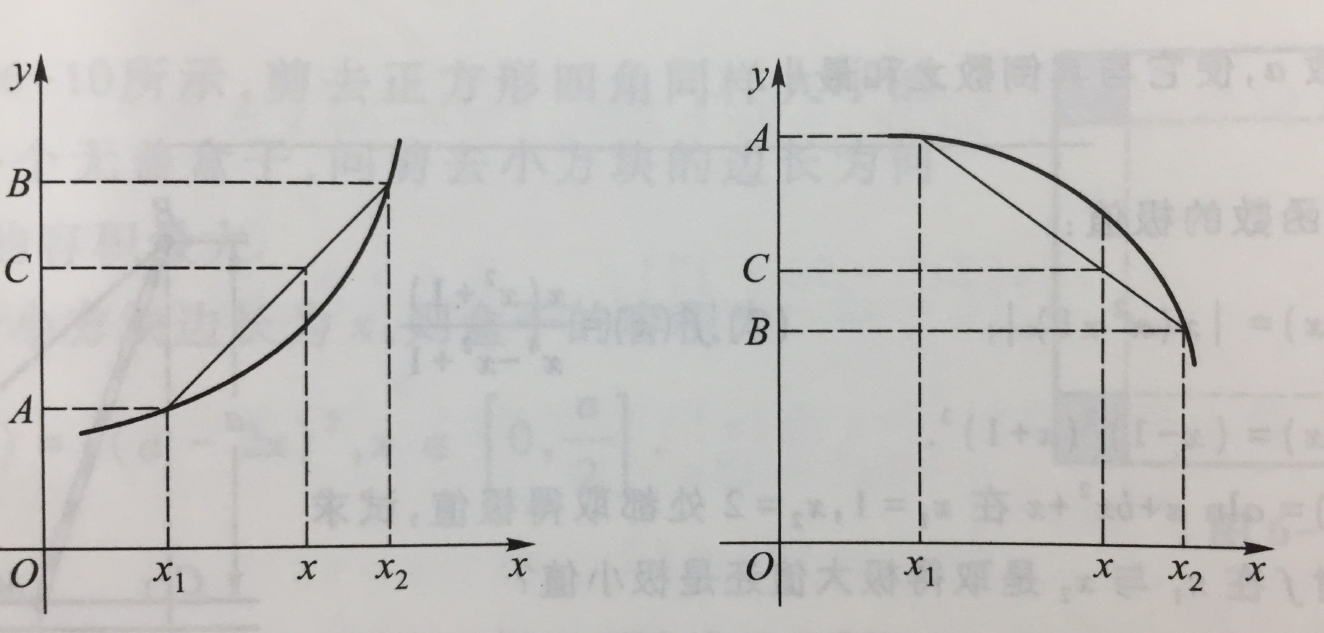
\includegraphics[width=0.48\linewidth,height=\textheight,keepaspectratio]{note-images/w4-convex.png}\par
\vspace{3pt}
{\small \emph{Lecture 12, p.25. Convex = below chords = concave up.}\par}
\end{minipage}
\end{center}

For \(x^2\), the left side minus the right side is
\(-\alpha(1-\alpha)(x-y)^2<0\) when \(x\ne y\).

\textbf{Ex.1.2.41 (Three-point criterion).} Convexity is equivalent to
\[
\frac{f(v)-f(u)}{v-u}\le\frac{f(w)-f(v)}{w-v}\quad(u<v<w).
\] Proof: write \(v=\alpha u+(1-\alpha)w\), \(\alpha=(w-v)/(w-u)\), and
rearrange the chord inequality. Strict version uses \(<\).

\textbf{Ex.1.2.42, 42'.} For differentiable \(f\) on an open interval,
\[
f\text{ convex}\iff f'\text{ nondecreasing},\qquad
f\text{ strictly convex}\iff f'\text{ strictly increasing}.
\] Reverse direction: MVT on \([u,v]\), \([v,w]\) turns the two slopes
into \(f'(\xi_1),f'(\xi_2)\) with \(\xi_1<\xi_2\).

Forward, strict case: fix \(u<z<v\) and shrink exterior secants: \[
f'(u)\le\frac{f(z)-f(u)}{z-u}<\frac{f(v)-f(z)}{v-z}\le f'(v).
\] Keep the middle strict inequality; limits alone may lose strictness.
Non-strict case: replace \(<\) by \(\le\).

\Needspace{5\baselineskip}
\textbf{Proposition 1.2.11.} For twice-differentiable \(f\),
\(f''\ge0\Rightarrow\) convex. If \(f''\ge0\) with \(f''>0\) except at
finitely many points, then strictly convex. Reverse signs for concavity.

Proof: MVT makes \(f'\) nondecreasing; in the second case it strictly
increases on a subinterval between any two points. Apply Ex.1.2.42.

Another proof idea: add \(\varepsilon x^2\), obtain strict convexity,
then let \(\varepsilon\downarrow0\) in the chord inequality.

\textbf{Ex.1.2.43-44.}

\begin{itemize}
\tightlist
\item
  \(x^{2n}\) on \(\mathbb R\) and \(x^n\) on \((0,\infty)\) (\(n>1\)):
  strictly convex. Also \(1/x\) on \((0,\infty)\); \(\sin x\) strictly
  concave on \([0,\pi]\).
\item
  \(x^{4/3}\): \(f'=\frac43x^{1/3}\) strictly increasing even across
  \(0\). Strictly convex, though \(f''(0)\) undefined.
\item
  \(x^{5/3}\): \(f'=\frac53x^{2/3}\) decreases left of \(0\), increases
  right. Concave down / up.
\end{itemize}
\end{document}
